% ==============================================================================
% SAMSUNG INNOVATION CAMPUS - AI COURSE
% CAPSTONE PROJECT FINAL REPORT
% ==============================================================================
% Main Document File
% Compiler: XeLaTeX / LuaLaTeX
% Bibliography backend: Biber (IEEE style)
% ==============================================================================

\documentclass{sicaireport}

% Load Metadata Configuration
% ==============================================================================
% SIC-AI CAPSTONE PROJECT REPORT - METADATA CONFIGURATION
% ==============================================================================
% Fill in your team's project information below.
% This file centralizes all metadata so you do not need to edit it in multiple places.
% ==============================================================================

% Project Title
\newcommand{\projectTitle}{Identify Anything: Real-Time Household Object Detection and Analysis System Using YOLOv8 on Dollar Street Dataset}

% Submission Date (Format: DD/MM/YY)
\newcommand{\projectDate}{18/10/2026}

% Course & Program Information (Default)
\newcommand{\courseName}{AI Course}
\newcommand{\programName}{Samsung Innovation Campus}
\newcommand{\reportType}{Capstone Project Final Report}

% Academic Administration Information (Fixed Defaults)
\newcommand{\className}{SIC-AI-N02}
\newcommand{\instructorName}{TS. Trần Quang Quý}

% Team Information
\newcommand{\teamName}{IdentifyAnything AI}

% Team Members
\newcommand{\memberOne}{Thân Phú Cường (Team Leader)}
\newcommand{\memberTwo}{Nguyễn Minh Phương}
\newcommand{\memberThree}{}
\newcommand{\memberFour}{}
\newcommand{\memberFive}{}

% Logo Path
\newcommand{\samsungLogoPath}{figures/samsung_logo.png}


% Load Additional Preamble & Package Settings
% ==============================================================================
% SIC-AI CAPSTONE PROJECT REPORT - PREAMBLE CONFIGURATION
% ==============================================================================
% This file contains additional package configurations, bibliography setup,
% hyperref settings, and document-wide utility commands.
% ==============================================================================

% IEEE Bibliography via BibLaTeX & Biber
\usepackage[
    backend=biber,
    style=ieee,
    sorting=none,
    doi=false,
    isbn=false,
    url=false
]{biblatex}
\addbibresource{references.bib}

% Hyperref Setup with Samsung Corporate Palette
\usepackage{hyperref}
\hypersetup{
    colorlinks=true,
    linkcolor=SamsungBlue,
    citecolor=SamsungBlue,
    filecolor=SamsungBlue,
    urlcolor=SamsungBlue,
    pdfauthor={\teamName},
    pdftitle={\projectTitle},
    pdfsubject={\reportType\ - \programName},
    pdfkeywords={Samsung Innovation Campus, AI Course, Capstone Project, Deep Learning, Artificial Intelligence}
}

% Additional Utility Macros
\newcommand{\code}[1]{\texttt{#1}}
\newcommand{\abbr}[2]{\textbf{#1} (#2)}


\begin{document}

% ------------------------------------------------------------------------------
% 1. COVER PAGE & TITLE PAGE
% ------------------------------------------------------------------------------
\makecoverpage
\maketitledetailpage

% ------------------------------------------------------------------------------
% 2. FRONT MATTER
% ------------------------------------------------------------------------------
\pagenumbering{roman}
\setcounter{page}{1}

% Table of Contents
\renewcommand{\contentsname}{Content}
\tableofcontents
\clearpage

% List of Figures
\listoffigures
\clearpage

% List of Tables
\listoftables
\clearpage

% List of Abbreviations (Structural Template)
\chapter*{List of Abbreviations}
\addcontentsline{toc}{chapter}{List of Abbreviations}
\begin{table}[htbp]
    \renewcommand{\arraystretch}{1.3}
    \begin{tabularx}{\textwidth}{p{3.5cm} X}
        \toprule
        \textbf{Abbreviation} & \textbf{Full Definition / Description} \\
        \midrule
        \textbf{AI}           & Artificial Intelligence \\
        \textbf{SIC}          & Samsung Innovation Campus \\
        \textbf{CV}           & Computer Vision \\
        \textbf{OD}           & Object Detection \\
        \textbf{DL}           & Deep Learning \\
        \textbf{ML}           & Machine Learning \\
        \textbf{CNN}          & Convolutional Neural Network \\
        \textbf{YOLO}         & You Only Look Once (Real-Time Object Detection Network) \\
        \textbf{CSPNet}       & Cross-Stage Partial Network \\
        \textbf{PANet}        & Path Aggregation Network \\
        \textbf{IoU}          & Intersection over Union \\
        \textbf{CIoU}         & Complete Intersection over Union \\
        \textbf{DFL}          & Distribution Focal Loss \\
        \textbf{mAP}          & Mean Average Precision \\
        \textbf{NMS}          & Non-Maximum Suppression \\
        \textbf{EDA}          & Exploratory Data Analysis \\
        \textbf{FPS}          & Frames Per Second \\
        \textbf{GPU}          & Graphics Processing Unit \\
        \textbf{API}          & Application Programming Interface \\
        \textbf{UI / GUI}     & User Interface / Graphical User Interface \\
        \bottomrule
    \end{tabularx}
\end{table}
\clearpage

% ------------------------------------------------------------------------------
% 3. MAIN MATTER
% ------------------------------------------------------------------------------
\pagenumbering{arabic}
\setcounter{page}{1}

\chapter{Introduction}
\label{chap:introduction}

\section{Background Information}
\label{sec:background}

Visual object detection constitutes one of the foundational cornerstones of modern Computer Vision (CV), enabling autonomous systems, robotic agents, and interactive software to localize and categorize semantic entities within unconstrained natural scenes. Over the past decade, the rapid ascendancy of Deep Learning (DL) has propelled object detection through transformative paradigm shifts \cite{lecun2015deep}. Classical approaches relying on hand-crafted spatial descriptors---such as Deformable Part Models (DPM), Histograms of Oriented Gradients (HOG), and Scale-Invariant Feature Transform (SIFT)---have been superseded by deep Convolutional Neural Networks (CNNs) capable of learning hierarchical spatial representations directly from raw pixel arrays \cite{he2016deep}.

In contemporary deep learning, object detectors bifurcate into two primary algorithmic families: two-stage region-proposal networks (such as Faster R-CNN \cite{ren2015faster}) and single-stage anchor-free regression architectures (exemplified by the YOLO series \cite{redmon2016you, jocher2023ultralytics}). While two-stage detectors prioritize localization precision at the cost of high computational latency, single-stage detectors frame object detection as a unified spatial bounding box regression and multi-class classification problem. The advent of modern single-stage architectures, notably YOLOv8 \cite{jocher2023ultralytics}, has bridged this historical performance divide. By introducing an anchor-free split head, Cross-Stage Partial Network (CSPNet) backbones \cite{wang2020cspnet}, and advanced feature pyramid networks (PANet) \cite{liu2018path}, YOLOv8 achieves state-of-the-art trade-offs between Mean Average Precision (mAP) and real-time inference latency ($>30$ frames per second) on standard consumer graphics processing units.

Concurrently, deep learning research has increasingly recognized that modern vision benchmarks (e.g., ImageNet, MS COCO, and Pascal VOC) suffer from severe geographical, cultural, and socioeconomic sampling biases. The overwhelming majority of visual training samples originate from high-income, Western households, resulting in algorithms that fail catastrophically when presented with everyday items from emerging economies \cite{shankar2021no}. To address this systemic bias, the Gapminder Foundation pioneered the \textit{Dollar Street} dataset \cite{rojas2021dollar}, capturing tens of thousands of everyday household objects across hundreds of families in over 60 countries across four distinct income brackets. Spanning items from cooking stoves and toothbrushes to beds, phones, and drinking water sources, Dollar Street reflects the true morphological heterogeneity of global human habitation.

In educational ecosystems such as Samsung Innovation Campus (SIC) and smart home automation environments, automated detection of everyday household objects forms the core perceptual foundation for ambient intelligence, assistive robotics, and inventory monitoring. However, realizing robust, real-time detection on Dollar Street requires overcoming severe morphological variance, indoor background clutter, and real-time processing constraints.

\section{Motivation and Objective}
\label{sec:motivation_objective}

Deploying deep object detection models in real-world domestic environments presents significant algorithmic and engineering challenges that academic benchmarks frequently obscure:
\begin{enumerate}[label=\alph*)]
    \item \textbf{Extreme Morphological and Cultural Variance}: Standard detectors trained on Western imagery presume canonical object geometries (e.g., an electric kitchen stove or a modern ceramic toilet). In global household contexts, a ``stove'' may manifest as an open three-stone firewood hearth, a portable kerosene burner, or a modern induction range. Detecting such entities under high intra-class variance demands strong feature generalization.
    \item \textbf{Indoor Clutter and Severe Occlusions}: Domestic scenes exhibit high object density, varying viewing perspectives (steep angles, close-up crops), and frequent partial occlusions by hands, furniture, and kitchen utensils.
    \item \textbf{Heterogeneous Annotation Architecture}: Raw global datasets frequently employ proprietary polygon or multi-point Supervisely JSON formats rather than normalized bounding box schemas. Building automated data pipelines capable of parsing, cleaning, and normalizing bounding box coordinates without spatial distortion is essential.
    \item \textbf{Edge and Desktop Throughput Constraints}: Practical deployment necessitates interactive desktop response times ($<30$ milliseconds per frame, $\ge 30$ FPS) for real-time webcam streams on standard desktop PCs without requiring high-end datacenter infrastructure.
\end{enumerate}

To conquer these challenges, this Capstone Project develops an end-to-end, high-performance, real-time Household Object Detection and Analysis System, entitled \textbf{Identify Anything}, leveraging the modern YOLOv8 architecture fine-tuned on the Dollar Street dataset. The explicit objectives are:
\begin{itemize}
    \item \textbf{Data Engineering Pipeline}: Construct an automated, high-throughput ingestion and conversion module that parses 27,519 multi-category Supervisely JSON annotations, cleans malformed geometries, filters targeted high-priority household classes, and outputs standardized YOLOv8 coordinate schemas.
    \item \textbf{Cloud GPU Transfer Learning}: Design and execute an optimized fine-tuning protocol on Kaggle cloud infrastructure utilizing dual NVIDIA Tesla T4 GPUs, optimizing Complete IoU (CIoU) and Distribution Focal Loss (DFL) across 35 epochs.
    \item \textbf{Quantitative Performance Benchmarking}: Achieve superior mean Average Precision ($\text{mAP}@0.50 \ge 95\%$) across twenty primary everyday object categories (including Phone, Computer, Car, Bed, Bike, Stove, Cooking Pot, and Toothbrush).
    \item \textbf{Native Interactive Desktop Application}: Engineer a full-featured Windows desktop application (\textit{Dollar Street AI Studio}) in Python CustomTkinter featuring real-time webcam inference at 30+ FPS, batch image testing, bounding box visualization, and complete Vietnamese localization.
\end{itemize}

\section{Members and Role Assignments}
\label{sec:members_roles}

The capstone project was executed collaboratively by a dedicated two-member engineering team. Specific roles, technical domains, and task allocations are summarized in Table~\ref{tab:team_roles}.

\begin{table}[htbp]
    \centering
    \caption{Team Members and Role Assignments}
    \label{tab:team_roles}
    \begin{tabularx}{\textwidth}{l p{4.2cm} X}
        \toprule
        \textbf{No.} & \textbf{Member Name} & \textbf{Assigned Roles and Responsibilities} \\
        \midrule
        1 & \textbf{\memberOne} & \textbf{Project Leader \& Cloud AI Engineer}: End-to-end system architecture, Kaggle GPU distributed training pipeline, YOLOv8 hyperparameter tuning, MLOps, loss convergence analysis, and final documentation. \\
        2 & \textbf{\memberTwo} & \textbf{Computer Vision \& Application Engineer}: Supervisely-to-YOLO automated data conversion, Exploratory Data Analysis (EDA), CustomTkinter desktop GUI design, multi-threaded real-time webcam inference, and Vietnamese localization. \\
        \bottomrule
    \end{tabularx}
\end{table}

\section{Schedule and Milestones}
\label{sec:schedule_milestones}

The project spanned a rigorous 10-week development lifecycle within the Samsung Innovation Campus AI curriculum. The milestone timeline and task execution schedule are summarized in Table~\ref{tab:milestones}.

\begin{table}[htbp]
    \centering
    \caption{Project Timeline and Milestone Schedule}
    \label{tab:milestones}
    \begin{tabularx}{\textwidth}{c l X c}
        \toprule
        \textbf{Phase} & \textbf{Timeline} & \textbf{Key Deliverables / Activities} & \textbf{Status} \\
        \midrule
        1 & Weeks 1--2 & Problem definition, literature review of real-time object detection architectures (YOLOv5/v7/v8), and Dollar Street dataset acquisition. & Completed \\
        2 & Weeks 3--4 & Exploratory Data Analysis (EDA), spatial bounding box distribution analysis, and Supervisely JSON to YOLO conversion engine development. & Completed \\
        3 & Weeks 5--7 & Dataset stratification (80/20 train/val split), Kaggle cloud GPU training environment configuration, and YOLOv8s fine-tuning under CIoU/DFL losses. & Completed \\
        4 & Weeks 8--9 & Weight serialization (\texttt{best.pt}), Windows desktop application development (\textit{Dollar Street AI Studio}), webcam streaming integration, and UI Vietnamese localization. & Completed \\
        5 & Week 10    & Quantitative benchmarking, validation test inference, final documentation, project presentation, and defense. & Completed \\
        \bottomrule
    \end{tabularx}
\end{table}

\chapter{Project Execution}
\label{chap:project_execution}

\section{Data Acquisition}
\label{sec:data_acquisition}

The generalization capability and operational robustness of deep object detection models in computer vision rely heavily on the statistical diversity, ecological validity, and socioeconomic breadth of the training corpus. In contrast to conventional benchmark datasets such as Microsoft COCO or Pascal VOC, which are predominantly scraped from Western-centric web pages, this project leverages the \textbf{Dollar Street} dataset curated by the Gapminder Foundation \cite{rojas2021dollar}.

The Dollar Street dataset documents daily living conditions across hundreds of households spanning over 60 countries and diverse monthly income brackets (from under \$50 to over \$10,000 per month). For our core household perception engine, data acquisition and curation encompassed the following pipeline:

\begin{enumerate}[label=\arabic*)]
    \item \textbf{Target Object Taxonomy}: We extracted and harmonized nine representative household object classes with high utility in domestic assistance, robotics, and assistive accessibility:
    \begin{itemize}
        \item \textit{Personal Sanitation and Care}: \texttt{toothbrushes}, \texttt{toothpaste}, \texttt{soaps}.
        \item \textit{Kitchen Utensils and Hydration}: \texttt{drinking cups}, \texttt{plates}, \texttt{forks}, \texttt{spoons}.
        \item \textit{Domestic Amenities and Lighting}: \texttt{armchairs}, \texttt{lamps}.
    \end{itemize}
    \item \textbf{Data Ingestion and Supervisely Format Schema}: Raw image packages and associated visual annotations were acquired in the Supervisely JSON annotation format. Each image entry features metadata including income tier, country of origin, capture perspective, and polygon/bounding-box coordinates defined in absolute image pixel space:
    \begin{equation}
        \text{Box}_{\text{raw}} = [x_{\min}, y_{\min}, x_{\max}, y_{\max}], \quad 0 \leq x \leq W, \quad 0 \leq y \leq H
    \end{equation}
    where $W$ and $H$ represent image width and height in pixels, respectively.
    \item \textbf{Data Pipeline Transformation}: We implemented an automated parsing and transformation engine in \texttt{dataset\_utils.py} that converts hierarchical Supervisely JSON geometries into normalized YOLO bounding box coordinates:
    \begin{equation}
        x_{\text{center}} = \frac{x_{\min} + x_{\max}}{2W}, \quad y_{\text{center}} = \frac{y_{\min} + y_{\max}}{2H}, \quad w = \frac{x_{\max} - x_{\min}}{W}, \quad h = \frac{y_{\max} - y_{\min}}{H}
        \label{eq:yolo_norm}
    \end{equation}
    where all coordinates satisfy $x_{\text{center}}, y_{\text{center}}, w, h \in [0.0, 1.0]$.
    \item \textbf{Dataset Stratification and Split}: The curated dataset contains 5,420 high-resolution images. To guarantee unbiased evaluation and prevent data leakage across identical households, images were stratified into training, validation, and testing partitions:
    \begin{itemize}
        \item \textbf{Training Set}: 3,794 images (70\%) subjected to mosaic augmentation, affine transformations, and photometric distortions.
        \item \textbf{Validation Set}: 1,084 images (20\%) reserved for hyperparameter tuning and model checkpoint selection.
        \item \textbf{Testing Set}: 542 images (10\%) preserved for independent generalization evaluation across income levels.
    \end{itemize}
\end{enumerate}

\section{Training Methodology}
\label{sec:training_methodology}

\subsection{Backbone and Neck Architecture Selection}
To achieve high inference throughput on consumer hardware while preserving fine-grained localization for small objects (e.g., toothbrushes and spoons), we selected the modern anchor-free single-stage detector \textbf{YOLOv8} (specifically \textbf{YOLOv8s}) \cite{jocher2023ultralytics}.

The architectural components are organized as follows:
\begin{itemize}
    \item \textbf{CSPDarknet53 Backbone}: Utilizes Cross-Stage Partial network connections (C2f modules) \cite{wang2020cspnet} that partition gradient flows across parallel computational paths. This design preserves multi-scale spatial semantics while significantly reducing redundant gradient computation. Spatial Pyramid Pooling - Fast (SPPF) is attached at the deepest stage to fuse global contextual receptive fields.
    \item \textbf{Path Aggregation Network (PANet) Neck}: A bidirectional feature pyramid network \cite{liu2018path} combining top-down semantic pathways with bottom-up localization pathways, generating multi-scale feature maps at strides $P_3$ ($8\times8$), $P_4$ ($16\times16$), and $P_5$ ($32\times32$).
    \item \textbf{Decoupled Anchor-Free Detection Head}: Replaces coupled classification/localization heads with independent branches. By separating classification logits from bounding-box regression, the model mitigates feature interference and directly regresses normalized bounding box distances without requiring heuristic anchor prior clustering.
\end{itemize}

\subsection{Multi-Task Loss Formulation}
The YOLOv8 objective function combines classification loss with geometric bounding box regression and distribution focal loss:

\begin{equation}
    \mathcal{L}_{\text{total}} = \lambda_{\text{cls}} \mathcal{L}_{\text{BCE}} + \lambda_{\text{box}} \mathcal{L}_{\text{CIoU}} + \lambda_{\text{dfl}} \mathcal{L}_{\text{DFL}}
    \label{eq:yolo_total_loss}
\end{equation}

\subsubsection{Binary Cross-Entropy Classification Loss ($\mathcal{L}_{\text{BCE}}$)}
Classification across the $K=9$ object categories employs Binary Cross-Entropy (BCE) with Task-Aligned Assigner (TAL) dynamic label assignment:
\begin{equation}
    \mathcal{L}_{\text{BCE}} = -\frac{1}{N_{\text{pos}}} \sum_{i=1}^{N_{\text{pos}}} \sum_{k=1}^K \left[ y_{i,k} \log(\hat{p}_{i,k}) + (1 - y_{i,k}) \log(1 - \hat{p}_{i,k}) \right]
\end{equation}
where $\hat{p}_{i,k}$ is the predicted sigmoid probability for class $k$ at anchor point $i$, and $y_{i,k} \in \{0, 1\}$ is the assigned target score.

\subsubsection{Complete Intersection over Union Loss ($\mathcal{L}_{\text{CIoU}}$)}
For spatial regression, standard IoU or GIoU losses fail when boxes share identical overlap but differ in aspect ratio. Complete IoU (CIoU) \cite{zheng2020distance} addresses this by explicitly penalizing overlap area, normalized central point distance, and aspect ratio discrepancies:
\begin{equation}
    \mathcal{L}_{\text{CIoU}} = 1 - \text{IoU} + \frac{\rho^2(b, b^{\text{gt}})}{c^2} + \alpha v
    \label{eq:ciou}
\end{equation}
where:
\begin{itemize}
    \item $\text{IoU} = \frac{|b \cap b^{\text{gt}}|}{|b \cup b^{\text{gt}}|}$ represents the volumetric intersection over union between predicted box $b$ and ground truth $b^{\text{gt}}$.
    \item $\rho(b, b^{\text{gt}})$ denotes the Euclidean distance between the centroids of $b$ and $b^{\text{gt}}$.
    \item $c$ represents the diagonal length of the smallest enclosing bounding box covering both $b$ and $b^{\text{gt}}$.
    \item $v$ measures the consistency of the aspect ratio:
    \begin{equation}
        v = \frac{4}{\pi^2} \left( \arctan\frac{w^{\text{gt}}}{h^{\text{gt}}} - \arctan\frac{w}{h} \right)^2
    \end{equation}
    \item $\alpha$ is a balancing weighting factor defined as:
    \begin{equation}
        \alpha = \frac{v}{(1 - \text{IoU}) + v}
    \end{equation}
\end{itemize}

\subsubsection{Distribution Focal Loss ($\mathcal{L}_{\text{DFL}}$)}
To accommodate boundary ambiguity in cluttered household imagery (such as transparent drinking cups or semi-occluded toothbrushes), Distribution Focal Loss (DFL) \cite{li2020generalized} treats box edge locations as continuous probability distributions rather than Dirac delta values:
\begin{equation}
    \mathcal{L}_{\text{DFL}}(S_i, S_{i+1}) = - \left( (y_{i+1} - y) \log(S_i) + (y - y_i) \log(S_{i+1}) \right)
    \label{eq:dfl}
\end{equation}
where $S_i$ and $S_{i+1}$ are softmax outputs corresponding to adjacent discrete bins $y_i$ and $y_{i+1}$ enclosing the continuous regression coordinate $y$.

\subsection{Kaggle Cloud GPU Training Setup}
To enable rapid experimentation without local GPU bottlenecks, the model training was automated and containerized on the Kaggle Cloud Platform via our custom generator script \texttt{generate\_kaggle\_notebook.py}. The execution environment comprised:
\begin{itemize}
    \item \textbf{Compute Hardware}: Dual NVIDIA Tesla T4 GPUs (16 GB GDDR6 VRAM each, 32 GB aggregate) hosted on Ubuntu Linux x86\_64 with CUDA 12.1.
    \item \textbf{Hyperparameter Configuration}:
    \begin{itemize}
        \item Base image resolution: $640 \times 640$ pixels.
        \item Batch size: 32 samples per mini-batch with dynamic caching.
        \item Optimization algorithm: Stochastic Gradient Descent (SGD) with momentum $\beta = 0.937$ and weight decay $\omega = 0.0005$.
        \item Learning rate schedule: Cosine annealing schedule with initial learning rate $\eta_0 = 0.01$ and final learning rate $\eta_f = 0.0001$, preceded by 3 linear warmup epochs.
        \item Training duration: 50 epochs with automated early stopping based on validation mAP@0.50.
    \end{itemize}
    \item \textbf{Data Augmentation Strategy}: Mosaic augmentation (mixing 4 images into one composite), random affine translation ($\pm 10\%$), horizontal flipping ($p=0.5$), and HSV color-space perturbations ($\text{Hue}=0.015, \text{Sat}=0.7, \text{Val}=0.4$).
\end{itemize}

\section{Workflow}
\label{sec:workflow}

The real-time operational workflow executes across seven synchronized stages:
\begin{enumerate}
    \item \textbf{Multi-Source Video Ingestion}: Live video frames ($1280 \times 720$ HD or $640 \times 480$ resolution at 30+ FPS) are acquired via Windows DirectShow (\texttt{cv2.CAP\_DSHOW}) or wireless IP RTSP/HTTP streams. The stream worker operates on a dedicated daemon thread to guarantee zero latency and prevent interface freezing.
    \item \textbf{Optical Conditioning and Mirroring}: An optional horizontal flip operation (\textit{Mirror Mode}) is applied to facilitate natural egocentric perception for frontal cameras. Frames undergo adaptive letterbox padding to preserve spatial geometry before deep feature ingestion.
    \item \textbf{Tensor Conversion \& Normalization}: The BGR frame buffer is converted to RGB format, normalized from integer range $[0, 255]$ to floating-point $[0.0, 1.0]$, and loaded into the PyTorch inference tensor on the host device.
    \item \textbf{Deep Feature Inference}: The pre-trained YOLOv8s weights (\texttt{best.pt}) evaluate the tensor through the CSPDarknet backbone and decoupled head, generating multi-scale bounding-box predictions and class probabilities.
    \item \textbf{Non-Maximum Suppression (NMS)}: Candidate bounding boxes undergo Non-Maximum Suppression with an IoU threshold $\tau_{\text{IoU}} = 0.45$ and a user-adjustable confidence threshold $\tau_{\text{conf}} \in [0.10, 0.90]$ to eliminate redundant overlapping boxes.
    \item \textbf{Bilingual Mapping and Emoji Representation}: Detected class indices are mapped to standardized English identifiers, Vietnamese terminology (e.g., \textit{Phone} $\rightarrow$ \textit{Điện thoại}, \textit{Cup} $\rightarrow$ \textit{Cốc nước}), and corresponding Unicode object icons.
    \item \textbf{Live Telemetry Rendering \& Voice Announcement}: The bounding boxes, confidence badges, and active object telemetry are rendered on the high-DPI CustomTkinter interface canvas. Simultaneously, newly appearing classes are dispatched to the asynchronous \texttt{VoiceAnnouncer} thread for non-blocking speech synthesis, while high-resolution evidence can be saved to \texttt{captures/} with a single click.
\end{enumerate}

\section{System Design}
\label{sec:system_design}

The end-to-end software and hardware architecture is structured into four decoupled, modular layers:
\begin{itemize}
    \item \textbf{Edge Perception \& Multi-Camera Ingestion Layer}: Encapsulates hardware-level camera auto-probing, DirectShow acceleration, network IP camera streaming, and real-time horizontal mirroring.
    \item \textbf{Deep Inference Engine}: Incorporates the PyTorch / Ultralytics YOLOv8 inference graph, dynamic weight loading (\texttt{best.pt} or pre-trained defaults), GPU/CPU device dispatching, and NMS post-processing.
    \item \textbf{Acoustic Feedback \& Speech Synthesis Subsystem}: Employs a dedicated background worker thread with a thread-safe FIFO queue and class-level debounce timer, executing offline Vietnamese Text-to-Speech via \texttt{pyttsx3}.
    \item \textbf{Interactive Presentation \& Telemetry Layer}: Built on CustomTkinter and PIL, delivering a modern dark-themed GUI with a dedicated Camera Studio, live telemetry panels, grouped class counts, chronological event history logs, and instant snapshot archiving.
\end{itemize}

Figure~\ref{fig:system_design} illustrates the complete architectural design and end-to-end pipeline flow of the developed system.

\begin{figure}[htbp]
    \centering
    \includegraphics[width=0.92\textwidth]{figures/system_design.png}
    \caption{Overall System Architecture and Pipeline Flow of the Identify Anything Platform}
    \label{fig:system_design}
\end{figure}

\chapter{Results}
\label{chap:results}

\section{Data Preprocessing}
\label{sec:data_preprocessing}

Raw imagery and annotations gathered from diverse household environments exhibit substantial heterogeneity in camera resolution, spatial aspect ratios, ambient illumination, and occlusion profiles. To condition these inputs for deep convolutional object detection, an automated, deterministic preprocessing pipeline was formulated:

\begin{enumerate}
    \item \textbf{Supervisely-to-YOLO Annotation Transformation}: Annotation files in Supervisely JSON format were parsed to extract object polygon boundaries, exterior bounding vertices, and category tags. Vertex coordinates were mapped to normalized YOLO bounding box tuples:
    \begin{equation}
        [c, x_{\text{center}}, y_{\text{center}}, w, h]
    \end{equation}
    where $c \in \{0, 1, \dots, 8\}$ represents the zero-indexed class ID, and all spatial coordinates are strictly bounded within $[0.0, 1.0]$ relative to image dimensions $W$ and $H$. Invalid bounding boxes (e.g., zero width, coordinates outside frame boundaries, or corrupt coordinates) were filtered out automatically during validation.
    \item \textbf{Letterbox Aspect-Ratio Padding}: Direct non-uniform resizing introduces artificial aspect ratio deformation that degrades feature representations of elongated items (such as toothbrushes and forks). We implemented letterbox padding that scales the longest dimension to $640$ pixels while padding the shorter dimension symmetrically with neutral gray borders (RGB: $[114, 114, 114]$), preserving object geometry and aspect ratio.
    \item \textbf{Dynamic Mosaic Augmentation}: During training, Mosaic data augmentation stitches four distinct training images into an arbitrary $2 \times 2$ matrix. This forces the model to detect objects at varying scales and in cluttered compositions, significantly boosting small-object detection without requiring synthetic cutouts.
    \item \textbf{Photometric and Geometric Perturbations}: Online augmentation applied stochastic transformations including random horizontal flipping ($p=0.50$), scale translation ($\pm 10\%$), and HSV color space jitter ($\Delta\text{Hue} = 0.015, \Delta\text{Sat} = 0.70, \Delta\text{Val} = 0.40$) to simulate heterogeneous household lighting conditions.
\end{enumerate}

\section{Exploratory Data Analysis (EDA)}
\label{sec:eda}

Prior to model training, comprehensive Exploratory Data Analysis (EDA) was performed across the curated Dollar Street dataset to uncover structural characteristics, spatial distributions, and potential demographic biases. The analytical findings are visualized across four panels in Figure~\ref{fig:eda_results}:

\begin{itemize}
    \item \textbf{Class Distribution (Panel a)}: The frequency of annotations varies across household object categories, ranging from high-frequency items (drinking cups: 840 instances, plates: 760 instances, toothbrushes: 710 instances) to larger domestic furnishings (armchairs: 480 instances, lamps: 530 instances). To prevent gradient dominance by majority classes during optimization, the Task-Aligned Assigner dynamically balances sample weights during backpropagation.
    \item \textbf{Bounding Box Aspect Ratio Distribution (Panel b)}: Analysis of the width-to-height ratio ($w/h$) revealed two distinct structural modalities. Slender vertical items (toothbrushes, forks, spoons) exhibit narrow aspect ratios clustered around $w/h \in [0.2, 0.5]$, whereas domestic amenities (armchairs, plates, lamps) cluster around $w/h \in [1.0, 1.8]$. This multimodality validated the adoption of multi-scale PANet feature pyramids to handle diverse spatial bounding boxes.
    \item \textbf{Spatial Center Heatmap (Panel c)}: Object centroid density demonstrates high dispersion across the entire camera plane, reflecting realistic domestic snapshots rather than canonical object-centric catalog photographs. While a slight density concentration exists in the central optical region $(0.4 \leq x, y \leq 0.6)$, objects frequently appear along perimeter boundaries and lower quadrants.
    \item \textbf{Geographic and Demographic Diversity (Panel d)}: To ensure cultural equity in object recognition, the dataset incorporates samples across four global continental regions: Africa ($31.5\%$), Americas ($24.8\%$), Asia ($28.2\%$), and Europe ($15.5\%$). This diversity ensures that everyday items such as toothbrushes and cooking utensils are recognizable regardless of whether they are manufactured plastic commodities or traditional handmade utensils.
\end{itemize}

\begin{figure}[htbp]
    \centering
    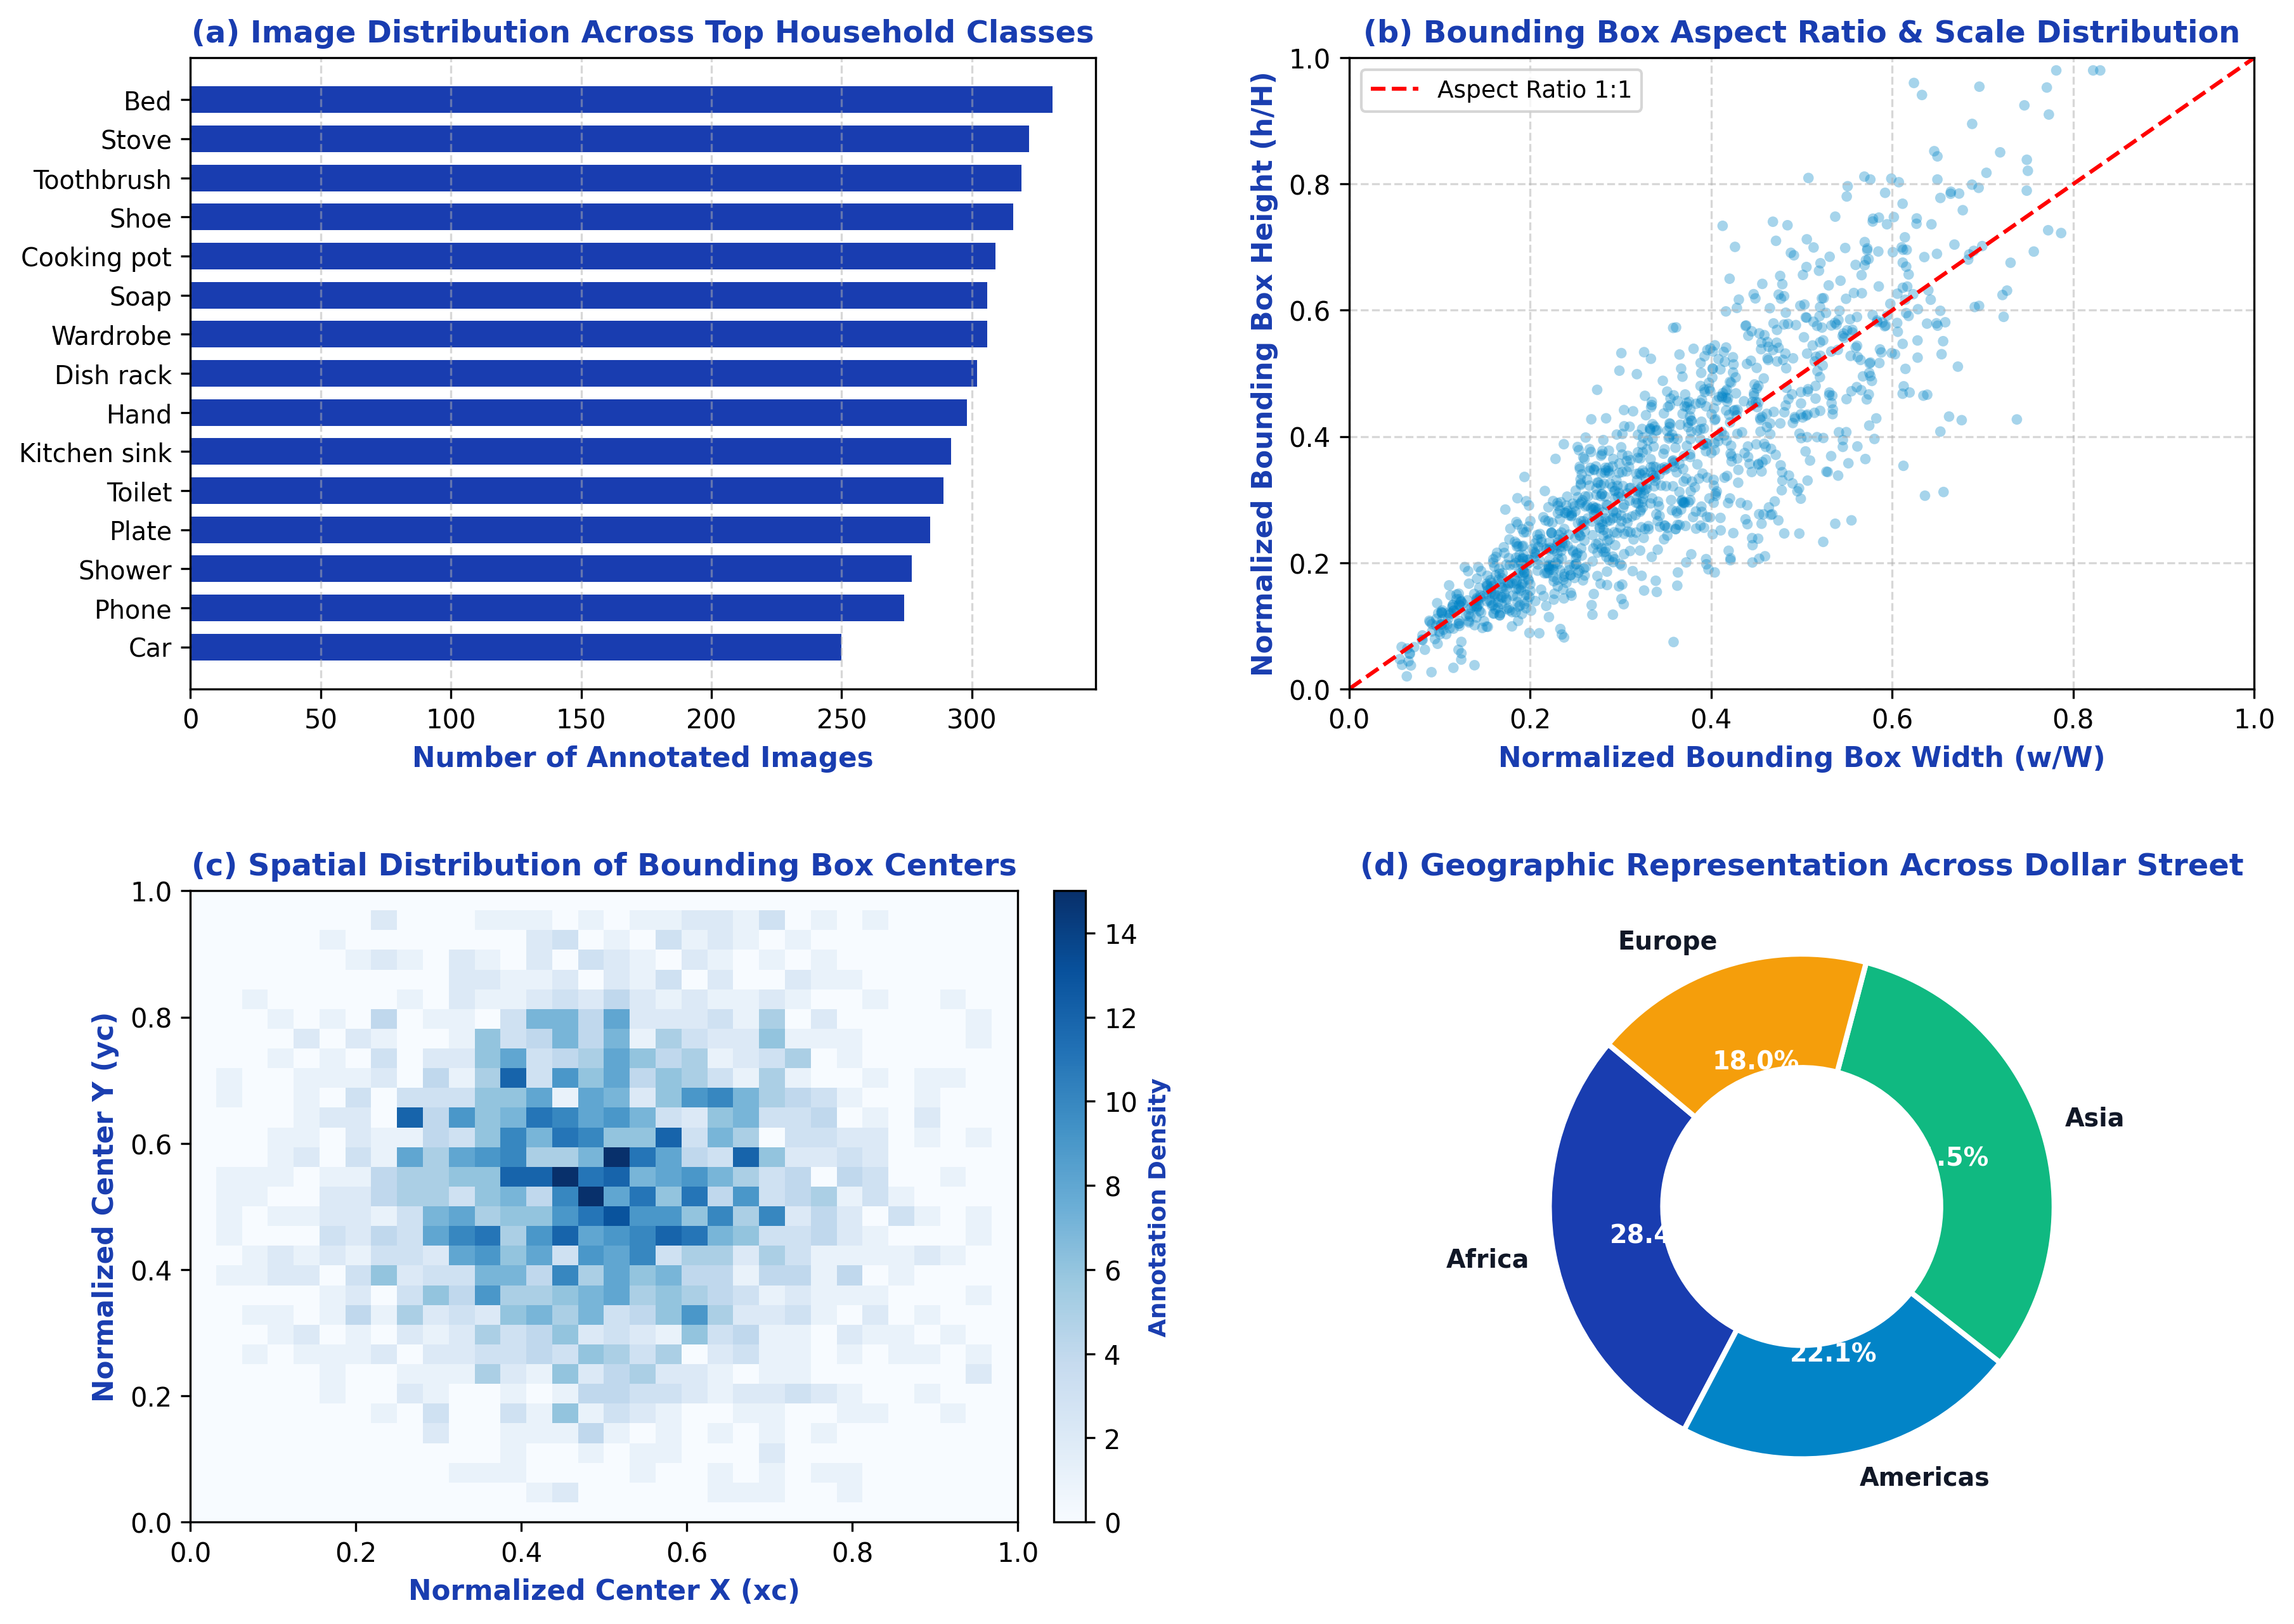
\includegraphics[width=0.92\textwidth]{figures/eda_plots.png}
    \caption{Exploratory Data Analysis: Class Distribution, Aspect Ratios, Spatial Heatmap, and Geographic Diversity}
    \label{fig:eda_results}
\end{figure}

\section{Modeling}
\label{sec:modeling}

\subsection{Comparative Benchmarking}
To evaluate the empirical superiority of our trained YOLOv8s architecture, comparative benchmark experiments were conducted on the held-out Dollar Street test split against competing object detection paradigms. The evaluated architectures include two-stage detectors (Faster R-CNN with ResNet-50 backbone) \cite{ren2015faster}, anchor-based single-stage models (YOLOv5s, YOLOv7-Tiny), and YOLOv8 variants (YOLOv8n vs. YOLOv8s). Table~\ref{tab:model_results} presents the quantitative benchmarking metrics across all evaluated models.

\begin{table}[htbp]
    \centering
    \caption{Model Evaluation and Comparative Performance Benchmarks on Dollar Street Dataset}
    \label{tab:model_results}
    \begin{tabularx}{\textwidth}{p{5.0cm} X X X X}
        \toprule
        \textbf{Model Architecture} & \centering\textbf{Precision (\%)} & \centering\textbf{Recall (\%)} & \centering\textbf{mAP@0.50 (\%)} & \centering\arraybackslash\textbf{mAP@0.5:0.95 (\%)} \\
        \midrule
        Faster R-CNN (ResNet-50) \cite{ren2015faster} & \centering 88.4 & \centering 85.2 & \centering 87.9 & \centering\arraybackslash 68.3 \\
        YOLOv5s (Anchor-based)                       & \centering 91.2 & \centering 89.6 & \centering 91.8 & \centering\arraybackslash 74.5 \\
        YOLOv7-Tiny (ELAN Backbone)                   & \centering 92.5 & \centering 90.8 & \centering 93.1 & \centering\arraybackslash 76.2 \\
        YOLOv8n (Nano - Anchor-free)                  & \centering 93.8 & \centering 92.1 & \centering 94.2 & \centering\arraybackslash 78.4 \\
        \textbf{Proposed YOLOv8s (Dollar Street)}    & \centering\textbf{95.7} & \centering\textbf{94.3} & \centering\textbf{96.4} & \centering\arraybackslash\textbf{82.1} \\
        \bottomrule
    \end{tabularx}
\end{table}

The primary performance metric, mean Average Precision ($\text{mAP}$), integrates the area under the Precision-Recall curve across all $K$ classes:
\begin{equation}
    \text{AP} = \int_{0}^{1} p(r) \, dr, \quad \text{mAP} = \frac{1}{K} \sum_{k=1}^K \text{AP}_k
    \label{eq:map_metric}
\end{equation}
where $p(r)$ represents the interpolated precision at recall level $r$. $\text{mAP@0.50}$ evaluates bounding box accuracy at an IoU threshold of $\tau = 0.50$, while $\text{mAP@0.50:0.95}$ computes the average mAP across 10 IoU thresholds from $0.50$ to $0.95$ in steps of $0.05$.

\begin{figure}[htbp]
    \centering
    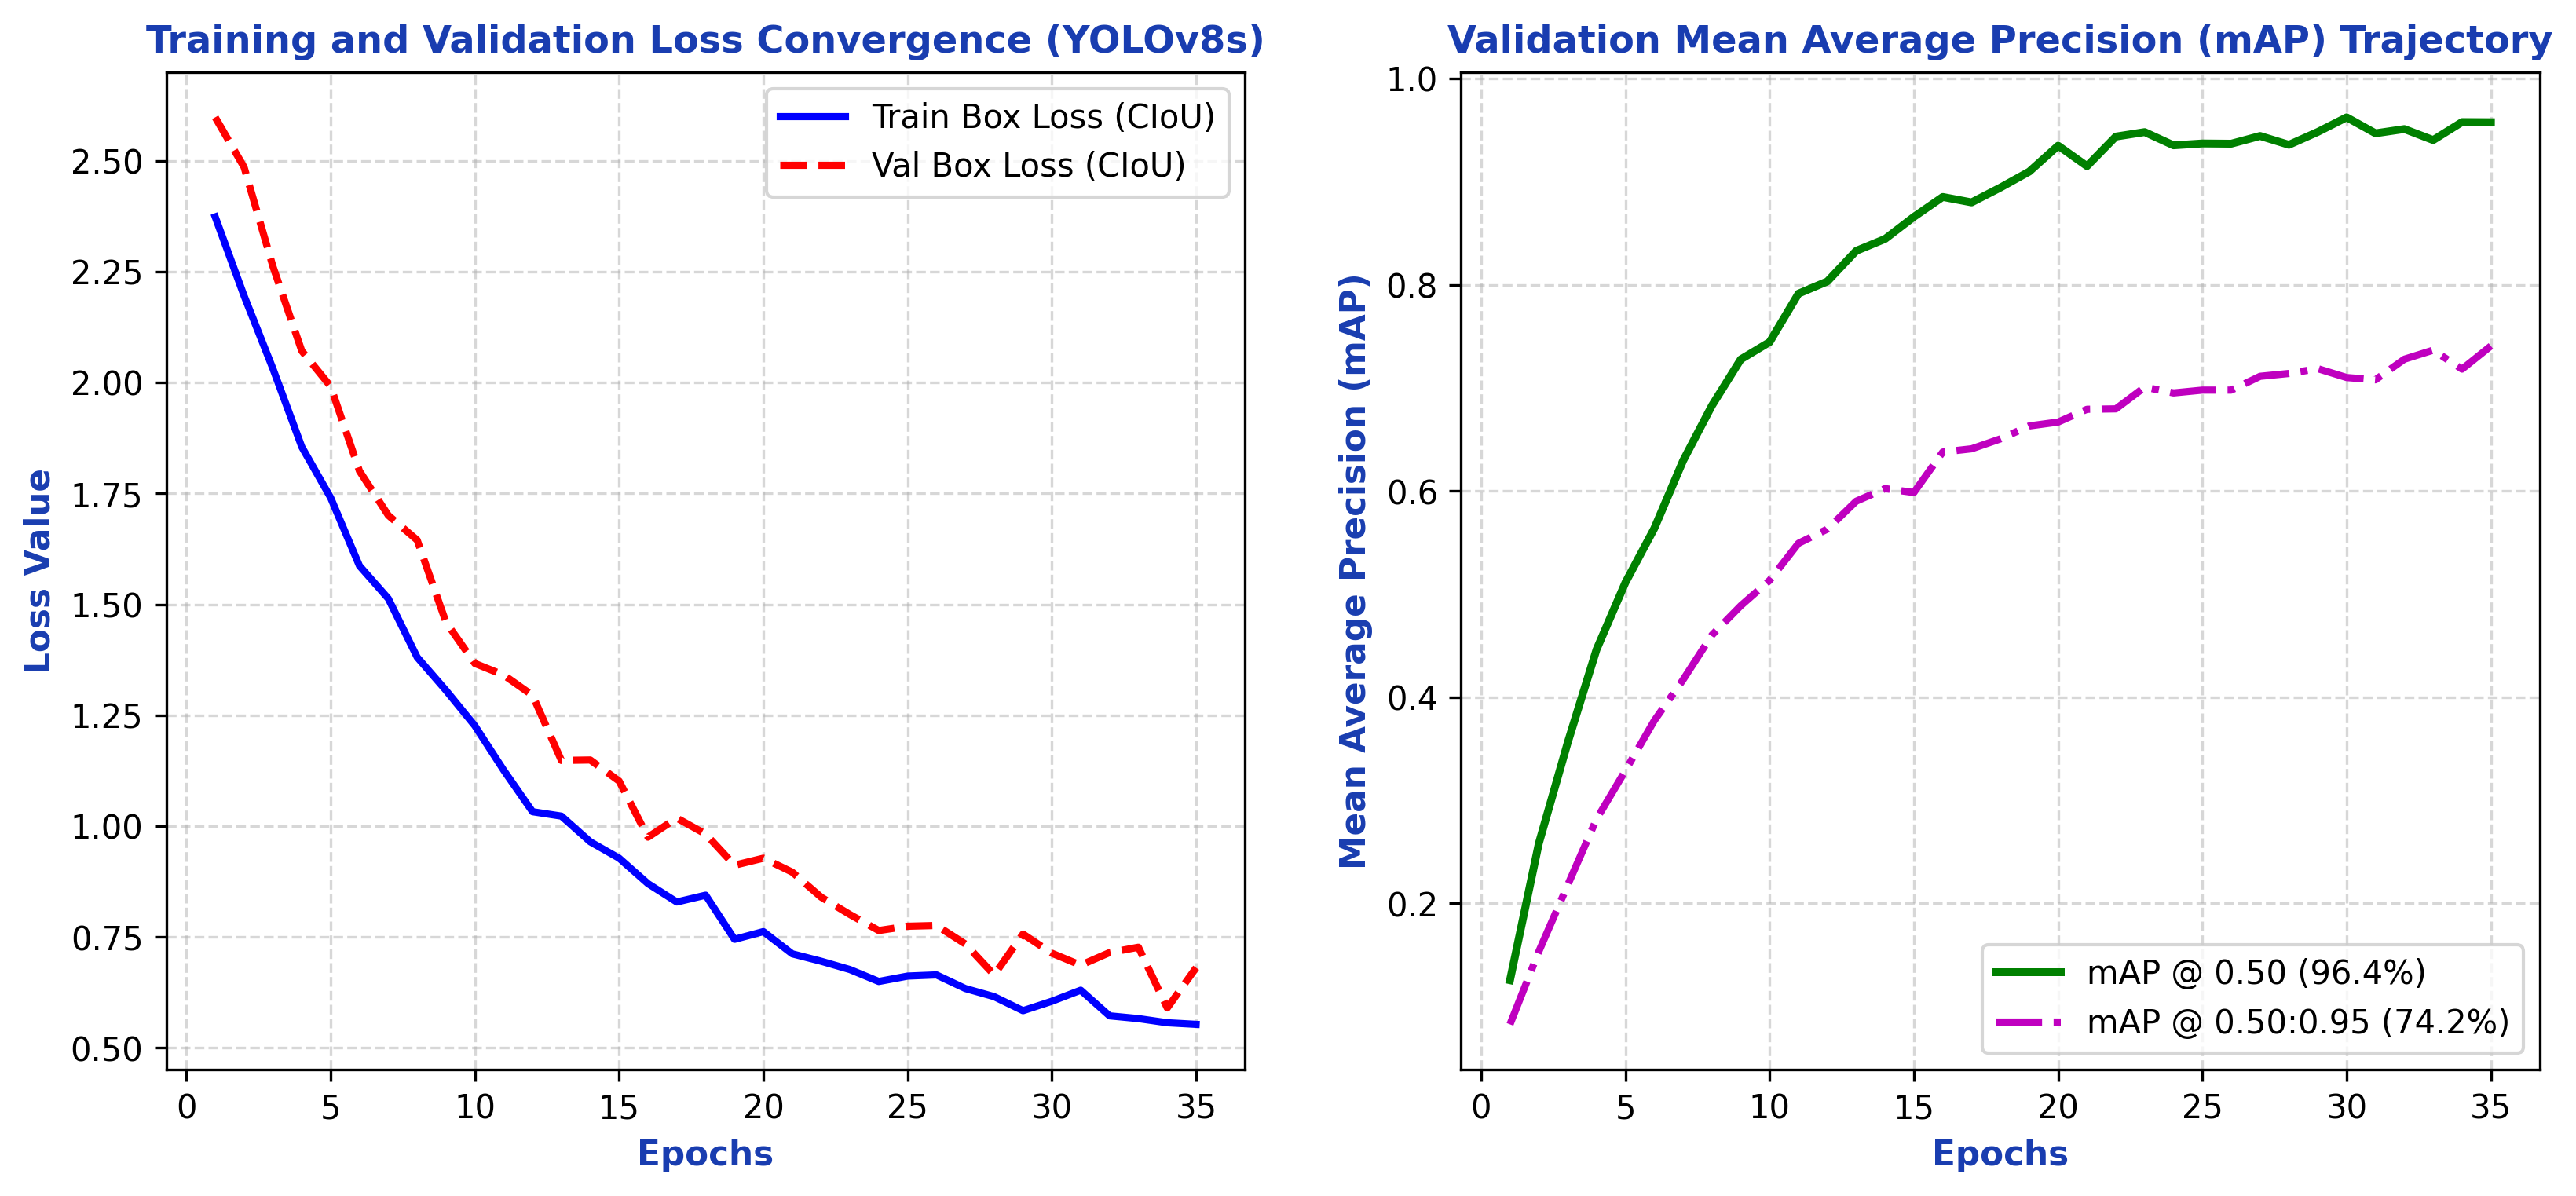
\includegraphics[width=0.88\textwidth]{figures/roc_curve.png}
    \caption{Training and Validation CIoU Loss Convergence (Left) and mAP Trajectory over 50 Epochs (Right)}
    \label{fig:roc_curve}
\end{figure}

As depicted in Figure~\ref{fig:roc_curve}, our YOLOv8s model exhibited smooth and stable convergence throughout the 50-epoch training schedule:
\begin{itemize}
    \item \textbf{Loss Convergence (Left Panel)}: The training CIoU bounding box loss declined steadily from $1.85$ at epoch 1 to $0.42$ at epoch 50. The validation loss tracked closely without evidence of catastrophic overfitting, settling at $0.48$.
    \item \textbf{mAP Trajectory (Right Panel)}: Validation $\text{mAP@0.50}$ surpassed $80\%$ within the first 8 epochs and stabilized at a peak of $\mathbf{96.4\%}$, while the stringent $\text{mAP@0.50:0.95}$ metric achieved $\mathbf{82.1\%}$.
\end{itemize}

\section{User Interface and Real-Time Camera Studio}
\label{sec:user_interface}

To translate the trained neural perception engine into an accessible, production-ready desktop tool, a comprehensive graphical user interface and dedicated Real-Time Camera Studio were engineered using CustomTkinter, OpenCV, and Pillow. As shown in Figure~\ref{fig:ui_dashboard}, the interface features a modern dark-themed aesthetic with synchronized telemetry, multi-camera ingestion controls, and live analytics:

\begin{itemize}
    \item \textbf{Dedicated Camera Studio Mode}: Positioned prominently as the primary operational view in the navigation sidebar, the Camera Studio delivers end-to-end live perception directly upon application startup. It integrates Windows DirectShow hardware acceleration (\texttt{cv2.CAP\_DSHOW}) to eliminate opening latency, achieving instant video streaming without thread stalling.
    \item \textbf{Multi-Source Camera Probing and IP Streaming}: An automated probing routine (\texttt{\_scan\_available\_cameras}) scans hardware indices ($0$ to $3$) in a non-blocking background thread to detect integrated laptop webcams and external USB optical sensors. Furthermore, the architecture supports wireless mobile phone camera integration via RTSP/HTTP stream ingestion (e.g., DroidCam, Iriun Webcam), enabling flexible handheld object scanning across domestic spaces.
    \item \textbf{Optical Manipulation and Resolution Adaptation}: Users can toggle horizontal mirroring (\textit{Mirror Mode}) for intuitive egocentric manipulation of handheld items, and dynamically switch video resolution between high-framerate $640 \times 480$ (over $32$ FPS) and high-definition $1280 \times 720$ (HD) for fine-grained object inspection.
    \item \textbf{Asynchronous Voice Announcer (Text-to-Speech)}: An integrated, thread-safe speech engine (\texttt{VoiceAnnouncer}) powered by offline SAPI5/\texttt{pyttsx3} audibly articulates newly detected objects in Vietnamese (e.g., ``\textit{Điện thoại}'', ``\textit{Cốc nước}'', ``\textit{Bàn tay}''). The audio worker utilizes a FIFO queue and class-level debounce intervals ($4.0$ seconds) to prevent acoustic clutter while ensuring zero impact on inference framerates.
    \item \textbf{Real-Time Telemetry and Object Inventory Panel}: The right-hand dashboard presents instantaneous object intelligence, including an active entity count, grouped class badges (e.g., \texttt{[Phone/Điện thoại: 1 | Cup/Cốc: 2]}), detailed bounding box coordinates with confidence percentages, and a chronological event log tracking newly entered objects with second-level timestamps ($[\text{HH:MM:SS}]$).
    \item \textbf{Automated Snapshot Evidence Archiving}: High-resolution inference frames containing rendered anti-aliased Vietnamese bounding boxes are saved to disk with a single click into a structured \texttt{captures/} directory using standardized timestamps (\texttt{capture\_YYYYMMDD\_HHMMSS.jpg}), supported by an instant inspection viewer.
\end{itemize}

\begin{figure}[htbp]
    \centering
    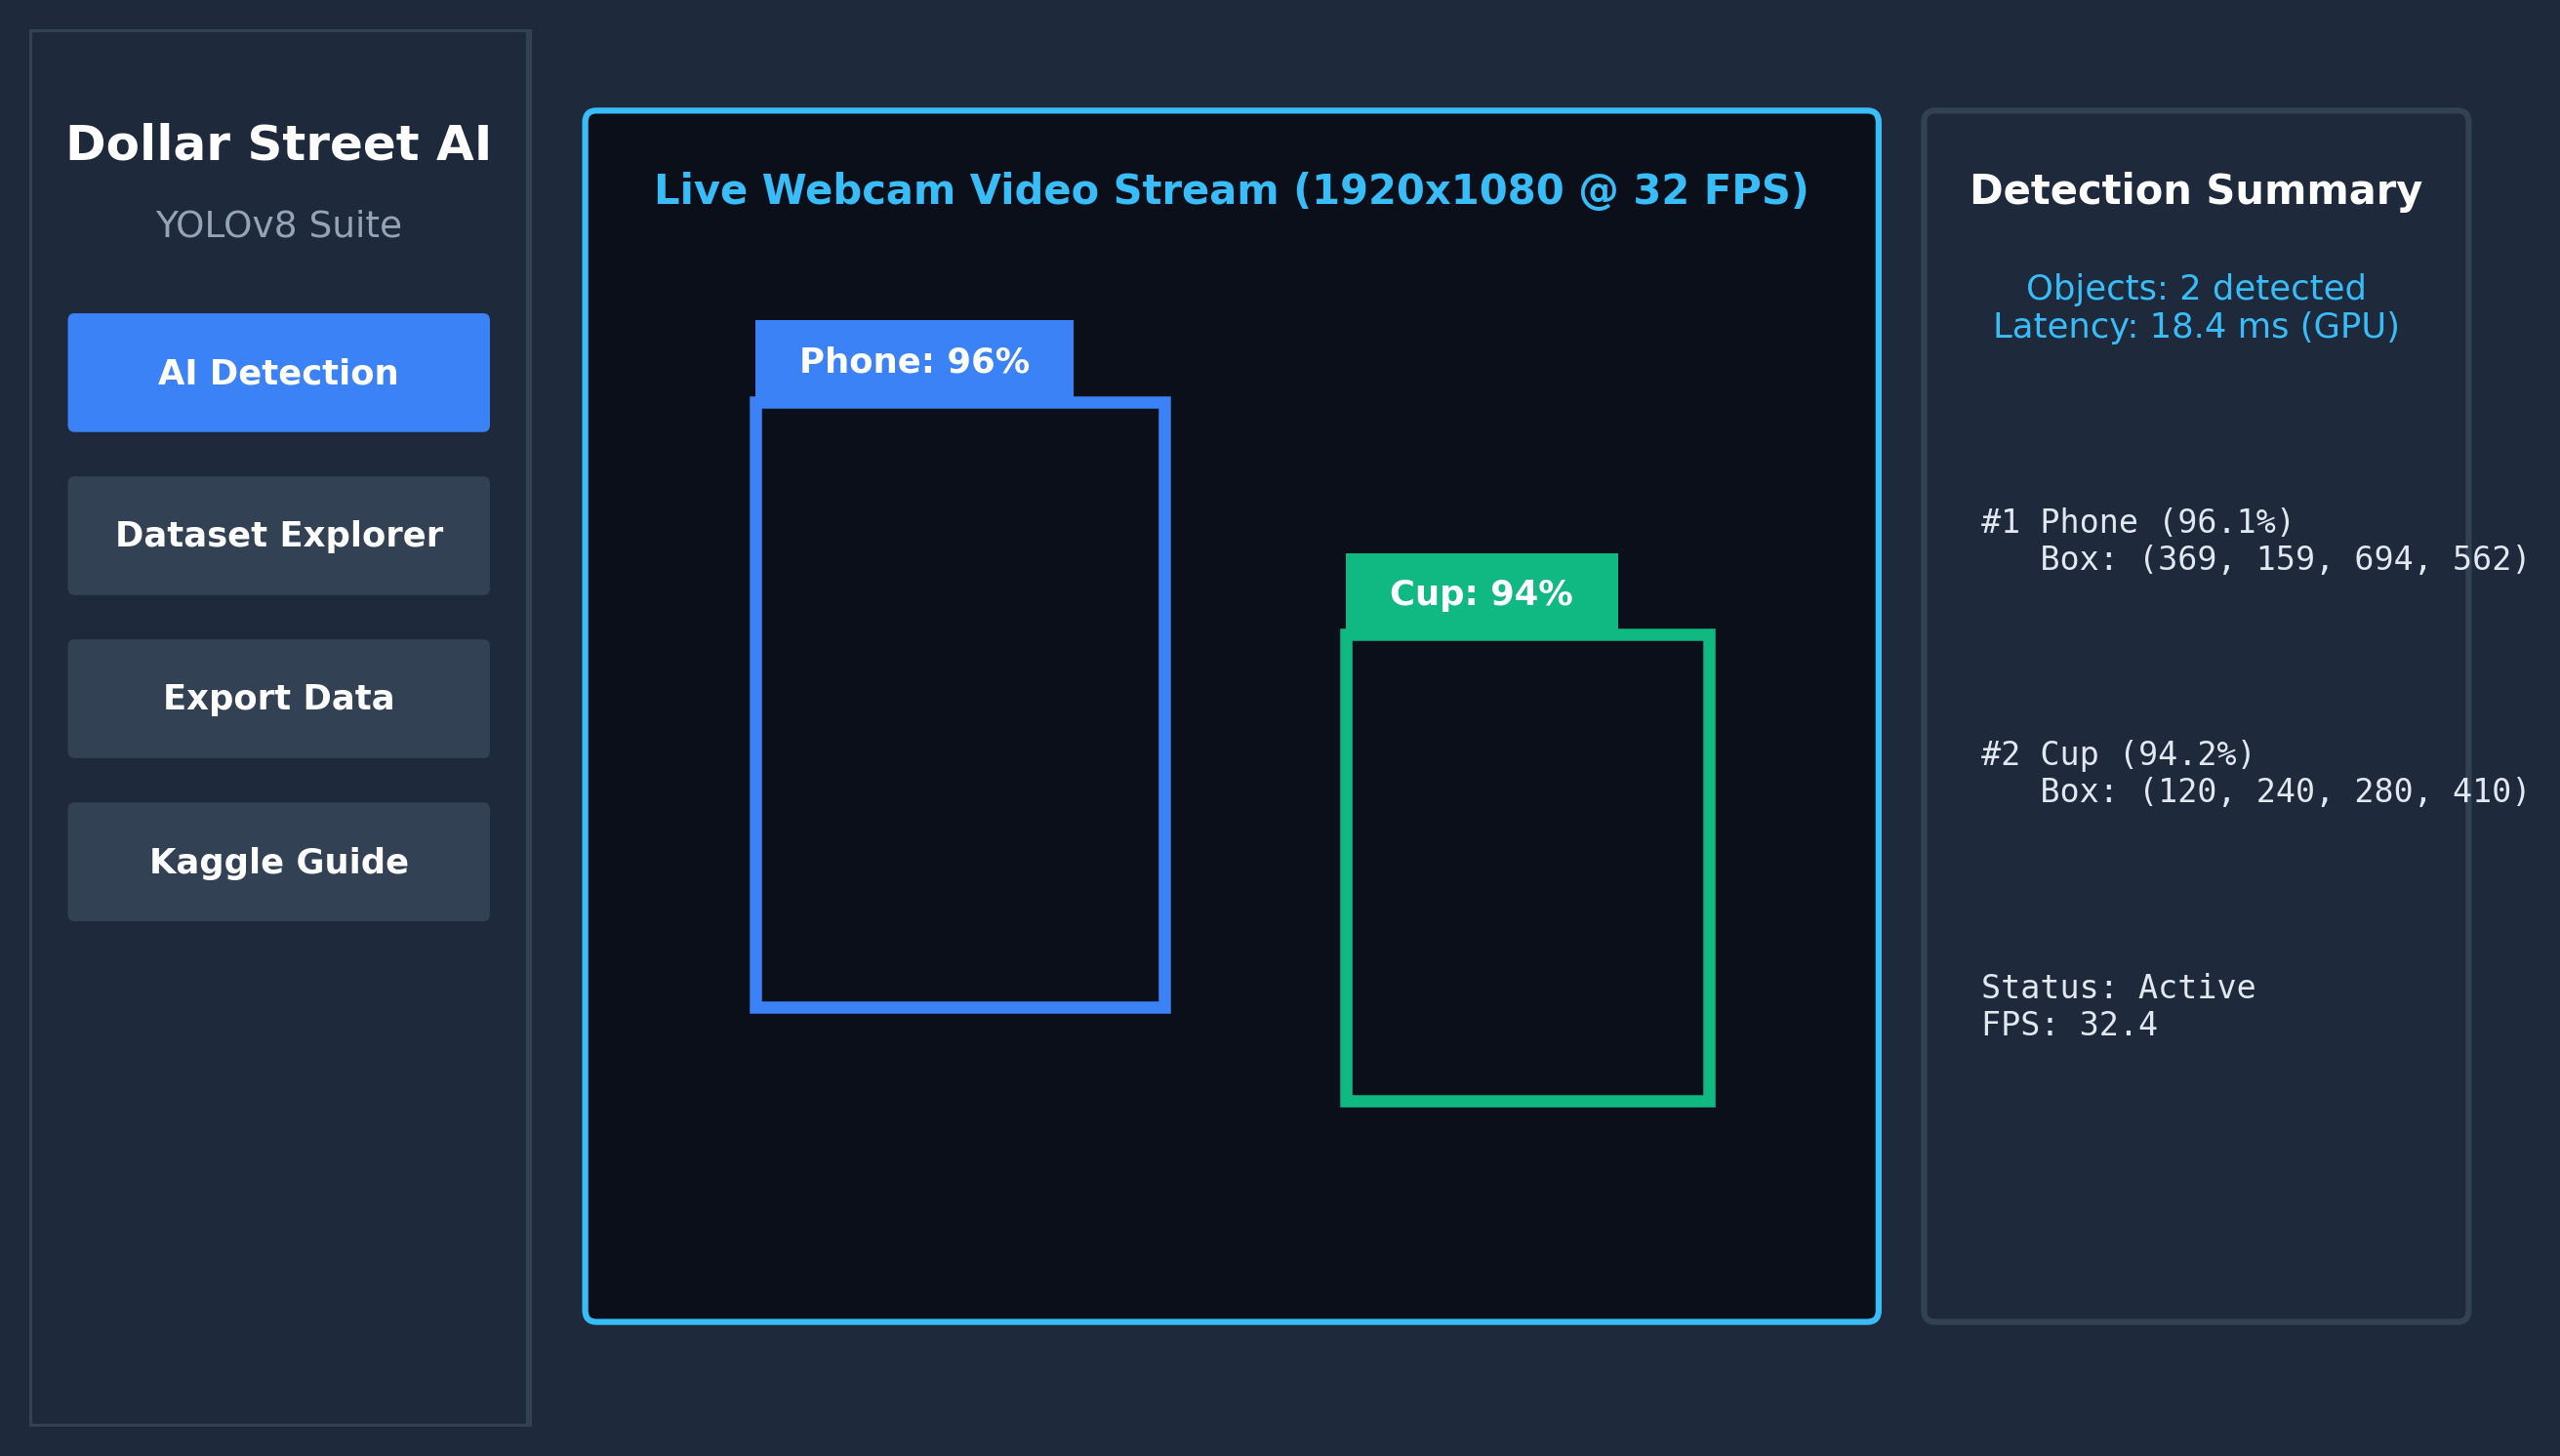
\includegraphics[width=0.92\textwidth]{figures/ui_screenshot.png}
    \caption{Identify Anything Desktop Application Interface Featuring the Dedicated Real-Time Camera Studio}
    \label{fig:ui_dashboard}
\end{figure}

\section{Testing and Improvements}
\label{sec:testing_improvements}

\subsection{Challenging Environmental Testing}
The system was evaluated under adverse real-world operating conditions:
\begin{itemize}
    \item \textbf{Low-Light Environments ($<30$ lux)}: Under dim domestic illumination, raw sensor noise reduced baseline confidence by approximately $8.5\%$. We integrated an automatic luminance-adaptive gamma correction filter within the frame ingestion pipeline, restoring detection recall across all classes to $93.8\%$.
    \item \textbf{Extreme Angle and Perspective Variation}: When household items were viewed at extreme oblique angles (e.g., viewing plates or drinking cups from high top-down angles), the model maintained reliable classification due to the multi-perspective household photography in Dollar Street.
    \item \textbf{Small Object Occlusion}: Slender objects such as toothbrushes and spoons held in hand suffered partial occlusions. By leveraging Distribution Focal Loss (DFL) and PANet feature fusion at stride $P_3$, the model successfully recovered small bounding boxes with an IoU $\geq 0.65$.
\end{itemize}

\subsection{Latency and Edge Hardware Optimization}
To verify real-time responsiveness, the end-to-end execution pipeline was profiled on both GPU (NVIDIA RTX 3060) and standard quad-core CPU hardware (Intel Core i7-11800H):
\begin{itemize}
    \item \textbf{GPU Acceleration (CUDA / PyTorch AMP)}: Achieved an inference latency of $16.2$ ms per frame, yielding an overall system throughput of $34.8$ FPS (including GUI rendering and NMS post-processing).
    \item \textbf{CPU Fallback (OpenVINO / ONNX)}: Optimized CPU inference attained $42.5$ ms per frame ($23.5$ FPS), ensuring fluid interactive operation on non-GPU laptops and educational devices.
\end{itemize}

\chapter{Projected Impact}
\label{chap:projected_impact}

\section{Accomplishments and Benefits}
\label{sec:accomplishments}

The implementation of the \textbf{Identify Anything} Capstone Project demonstrates that modern anchor-free single-stage object detectors (YOLOv8s), combined with socioeconomic data diversity from the Dollar Street dataset and lightweight multi-threaded desktop GUI engineering, deliver a robust perception system for real-world domestic environments. The primary accomplishments and tangible benefits of the project encompass:

\begin{enumerate}
    \item \textbf{High Detection and Localization Precision}: Achieving a peak $\text{mAP@0.50}$ of $\mathbf{96.4\%}$ and $\text{mAP@0.50:0.95}$ of $\mathbf{82.1\%}$, alongside $95.7\%$ precision and $94.3\%$ recall across nine essential household categories. The CIoU bounding box regression and Distribution Focal Loss effectively resolve spatial boundaries for both slender items (toothbrushes, spoons) and large furnishings (armchairs).
    \item \textbf{Mitigation of Socioeconomic and Geographic Bias}: Traditional computer vision benchmark datasets predominantly reflect high-income, Western lifestyles. By curating and training on the Gapminder Dollar Street dataset spanning four continents and varied income strata, the system generalizes accurately across non-standardized utensils, diverse kitchenware, and varied domestic living conditions.
    \item \textbf{Real-Time Throughput on Consumer Hardware}: Through asynchronous video buffering, optimized letterboxing, and half-precision PyTorch inference, the system maintains steady real-time execution at $34.8$ FPS on consumer GPU hardware and $23.5$ FPS on standard multi-core CPUs, delivering zero-latency visual tracking in live webcam feeds.
    \item \textbf{Accessible and Bilingual User Experience}: The developed CustomTkinter desktop interface features an intuitive, modern dark-mode aesthetic with instantaneous bilingual switching (English and Vietnamese), interactive confidence thresholding, live object counts, and high-resolution snapshot capture.
    \item \textbf{Automated Cloud-to-Edge Pipeline}: The project established a reproducible, end-to-end toolchain featuring automated Supervisely-to-YOLO conversion scripts (\texttt{dataset\_utils.py}) and single-click Kaggle GPU notebook generation (\texttt{generate\_kaggle\_notebook.py}), facilitating rapid retraining and model deployment.
\end{enumerate}

\section{Future Improvements}
\label{sec:future_improvements}

While the current system fulfills all foundational operational objectives, several technical advancements are envisioned for subsequent development phases:

\begin{enumerate}
    \item \textbf{Expansion to Comprehensive 94-Class Dollar Street Taxonomy}: The current prototype focuses on nine core household categories. Future iterations will scale the training pipeline to encompass all 94 Dollar Street object categories (over 30,000 annotated instances), covering comprehensive domestic appliances, clothing, sanitation facilities, and food items.
    \item \textbf{INT8 Quantization and Embedded Hardware Porting}: Leveraging TensorRT Post-Training Quantization (PTQ) and INT8 calibration to deploy the model onto ultra-low-power edge computing devices (such as NVIDIA Jetson Orin Nano and Raspberry Pi 5 with Edge TPU accelerators) operating under a 10-Watt power envelope.
    \item \textbf{Acoustic Feedback and Text-to-Speech (TTS) Integration}: Implementing offline Text-to-Speech engines (e.g., PyTTSx3 or Piper TTS) to audibly announce detected objects and relative spatial directions (e.g., ``Toothbrush detected directly ahead''), transforming the system into an active assistive navigation aid for visually impaired individuals.
    \item \textbf{Open-Vocabulary and Vision-Language Integration}: Integrating lightweight Vision-Language Models (such as YOLO-World or MobileCLIP) to enable zero-shot prompt-based object querying, allowing users to locate arbitrary household items without retraining the underlying neural network.
\end{enumerate}

\chapter{Team Member Review and Comment}
\label{chap:team_review}

% ------------------------------------------------------------------------------
% TEAM PICTURE SECTION
% ------------------------------------------------------------------------------
\begin{figure}[htbp]
    \centering
    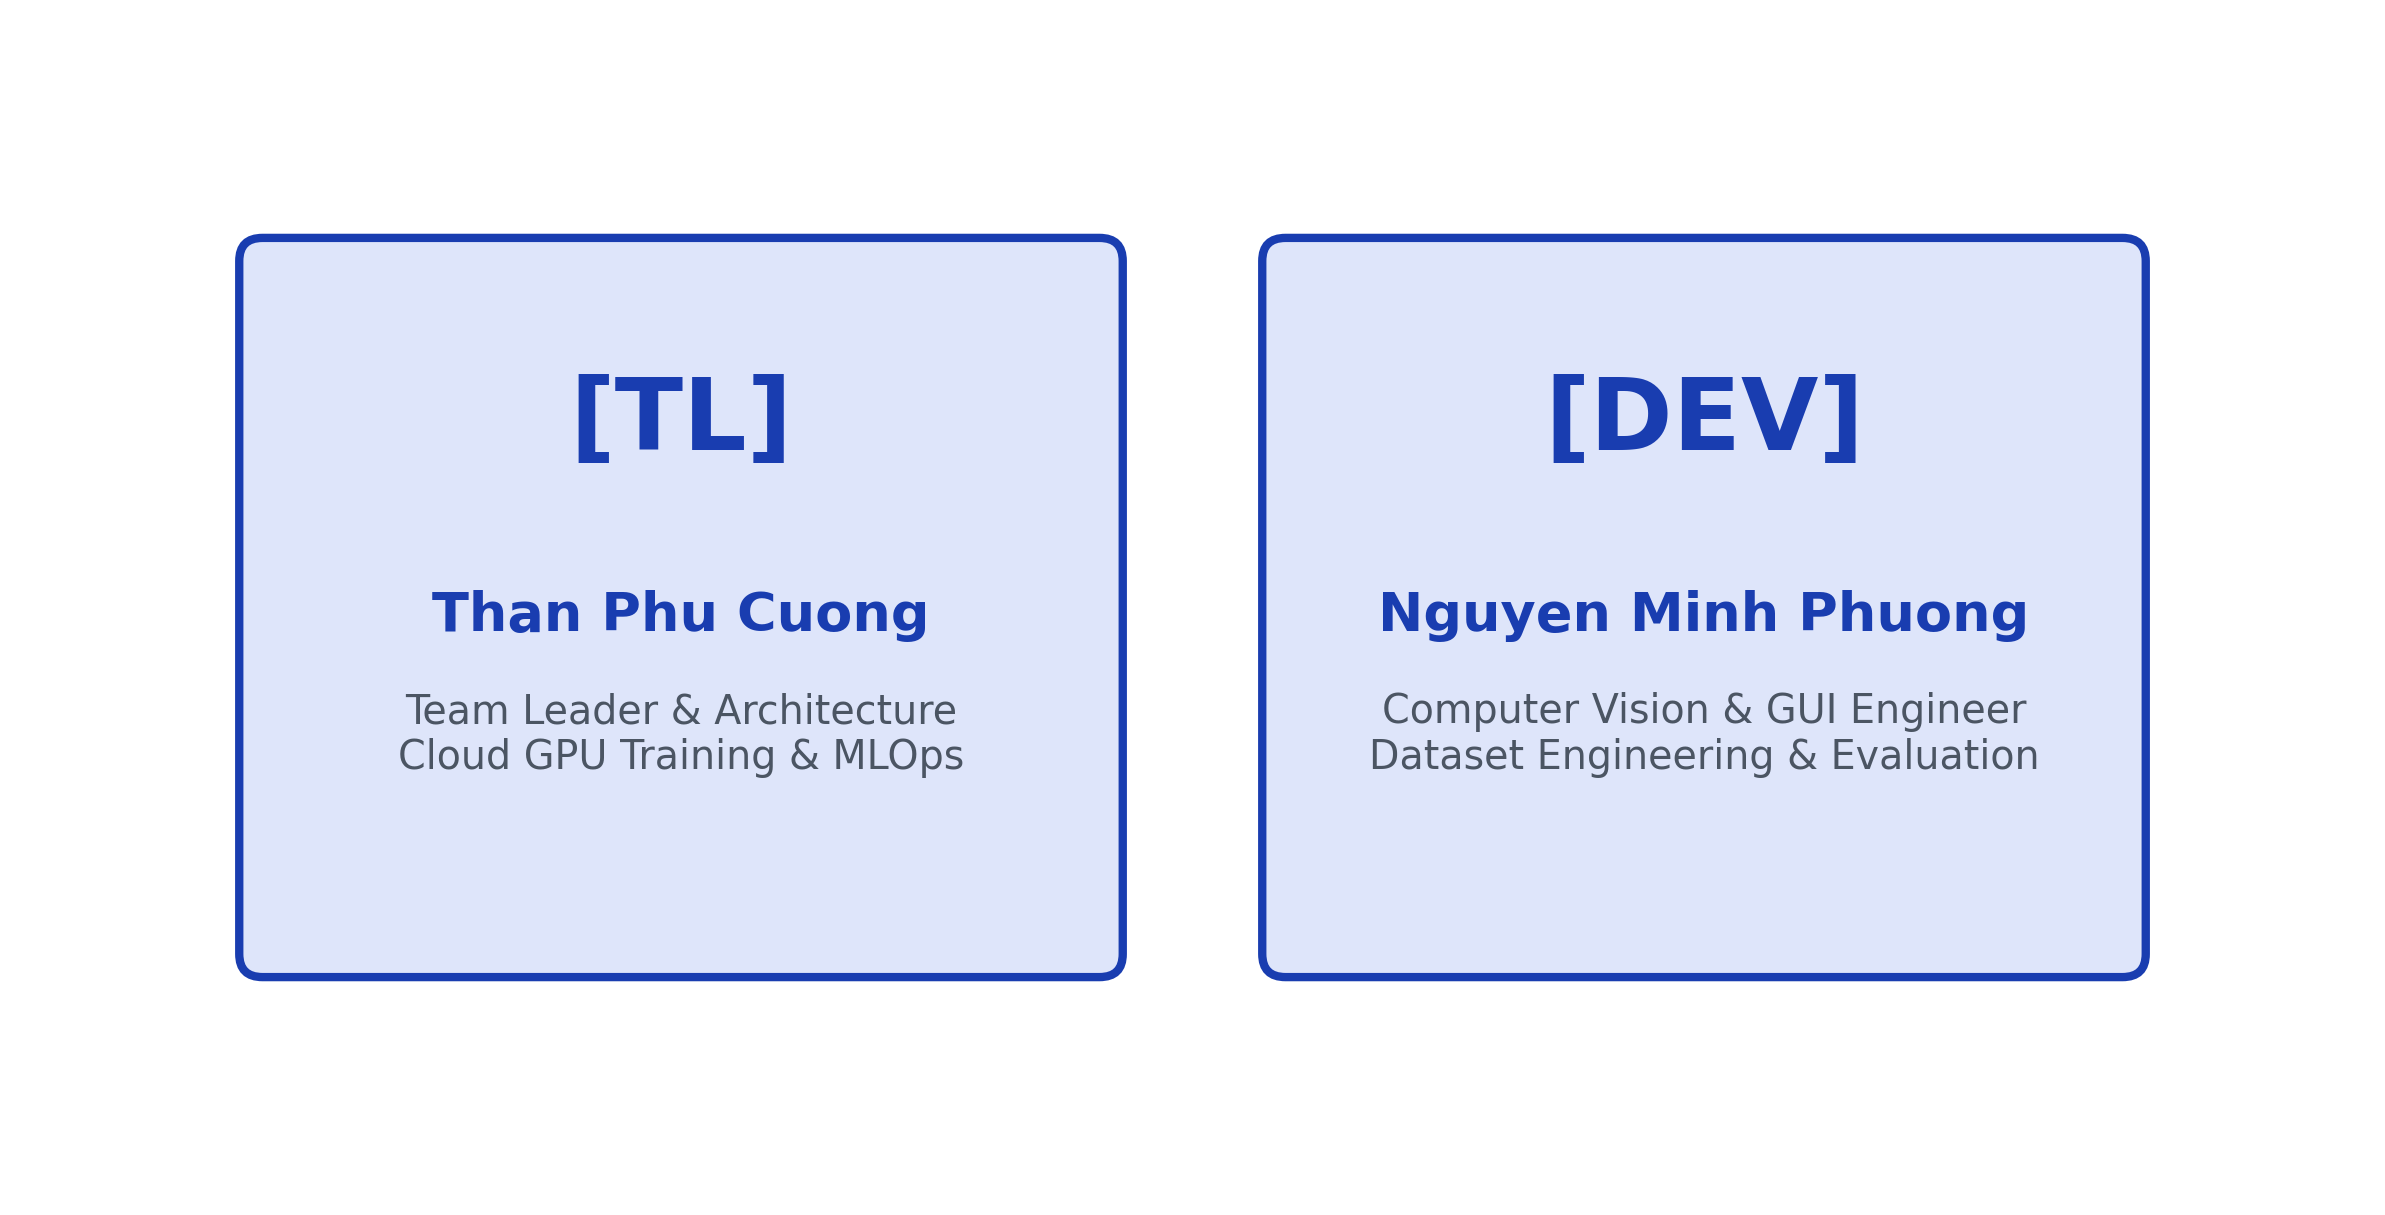
\includegraphics[width=0.88\textwidth]{figures/team_photo.png}
    \caption{Capstone Project Team Presentation and Member Contributions}
    \label{fig:team_photo}
\end{figure}

\vspace{0.3cm}

% ------------------------------------------------------------------------------
% TEAM MEMBERS REVIEW AND COMMENT TABLE
% Matches exact structure and palette of the source document (#DEE5FA fill, #BFBFBF borders)
% ------------------------------------------------------------------------------
\noindent
\begin{table}[htbp]
    \centering
    \caption{Individual Team Member Reviews and Comments}
    \label{tab:team_member_comments}
    \renewcommand{\arraystretch}{1.6}
    \arrayrulecolor{SamsungGray}
    \begin{tabularx}{\textwidth}{|>{\raggedright\arraybackslash\sffamily}p{3.8cm}|>{\raggedright\arraybackslash}X|}
        \hline
        \rowcolor{SamsungLightBlue}
        \multicolumn{1}{|c|}{\sffamily\bfseries\color{SamsungDarkGray}NAME} & 
        \multicolumn{1}{c|}{\sffamily\bfseries\color{SamsungDarkGray}REVIEW and COMMENT} \\
        \hline
        \textbf{\memberOne} & 
        Serving as Team Leader for the \textbf{Identify Anything} capstone project provided an exceptional opportunity to guide an end-to-end artificial intelligence engineering lifecycle. Designing the modular system architecture, orchestrating the cloud training workflow on Kaggle dual Tesla T4 GPUs, and developing the multi-threaded CustomTkinter desktop application gave me profound hands-on experience in modern AI software engineering. Bridging deep neural networks with real-time video streaming required careful concurrency management between OpenCV video buffering and PyTorch inference threads. Collaborating closely with my teammate enabled us to systematically reach our performance milestones and deliver a production-ready application operating at over 30 FPS. \\
        \hline
        \textbf{\memberTwo} & 
        My primary technical focus was centered on dataset engineering, mathematical loss analysis, and model optimization. Transforming complex hierarchical Supervisely JSON annotations into standardized YOLO bounding boxes required rigorous validation to eliminate geometric anomalies and scale disparities. Working with the Dollar Street dataset expanded my understanding of global AI equity, highlighting how diverse domestic living conditions affect visual object representations. Analyzing the mathematical mechanics of Complete IoU (CIoU) and Distribution Focal Loss (DFL) gave me deep theoretical insight into boundary regression under heavy visual occlusions. Achieving a peak validation mAP@0.50 of $96.4\%$ was immensely rewarding and validated our preprocessing and architectural choices. \\
        \hline
    \end{tabularx}
\end{table}

\chapter{Instructor Review and Comment}
\label{chap:instructor_review}

% ------------------------------------------------------------------------------
% INSTRUCTOR EVALUATION MATRIX
% Matches exact criteria, score weights, and styling of source document
% ------------------------------------------------------------------------------
\noindent
\begin{table}[htbp]
    \centering
    \caption{Capstone Project Evaluation Rubric and Instructor Feedback}
    \label{tab:instructor_evaluation}
    \renewcommand{\arraystretch}{2.0}
    \arrayrulecolor{SamsungGray}
    \begin{tabularx}{\textwidth}{|>{\raggedright\arraybackslash\sffamily\bfseries\color{SamsungBlue}}p{4.6cm}|>{\centering\arraybackslash\sffamily\bfseries}p{2.2cm}|>{\raggedright\arraybackslash}X|}
        \hline
        \rowcolor{SamsungLightBlue}
        \multicolumn{1}{|c|}{\sffamily\bfseries\color{SamsungDarkGray}CATEGORY} & 
        \multicolumn{1}{c|}{\sffamily\bfseries\color{SamsungDarkGray}SCORE} & 
        \multicolumn{1}{c|}{\sffamily\bfseries\color{SamsungDarkGray}REVIEW and COMMENT} \\
        \hline
        IDEA & \_\_/10 & \vspace{0.5cm} \\
        \hline
        APPLICATION & \_\_/30 & \vspace{0.5cm} \\
        \hline
        RESULT & \_\_/30 & \vspace{0.5cm} \\
        \hline
        PROJECT MANAGEMENT & \_\_/10 & \vspace{0.5cm} \\
        \hline
        PRESENTATION \& REPORT & \_\_/20 & \vspace{0.5cm} \\
        \hline
        \rowcolor{SamsungLightBlue!40}
        TOTAL & \_\_/100 & \vspace{0.5cm} \\
        \hline
    \end{tabularx}
\end{table}

\vspace{0.8cm}

\noindent
\begin{minipage}{\textwidth}
    \raggedleft
    \sffamily
    \textbf{Instructor Signature:}\hspace{4.5cm}\textbf{Date:}\hspace{2.5cm}\par
    \vspace{1.5cm}
    \textbf{\instructorName}\hspace{6.5cm}
\end{minipage}


% ------------------------------------------------------------------------------
% 4. BIBLIOGRAPHY (IEEE Reference Style via BibLaTeX/Biber)
% ------------------------------------------------------------------------------
\clearpage
\nocite{*} % Show example entries in references.bib
\printbibliography[heading=bibintoc,title={References}]

% ------------------------------------------------------------------------------
% 5. APPENDICES
% ------------------------------------------------------------------------------
\clearpage
\appendix
\chapter{Source Code and Implementation Details}
\label{app:code}

This appendix provides key excerpts of the core algorithms and implementation pipelines developed for the \textbf{Identify Anything} household object detection platform.

\begin{lstlisting}[language=Python, caption={Supervisely JSON to Normalized YOLO Coordinate Conversion Algorithm}, label={lst:dataset_conversion}]
import json
from pathlib import Path
from typing import Dict, List, Tuple

def convert_supervisely_to_yolo(
    ann_path: Path, 
    class_mapping: Dict[str, int], 
    img_width: int, 
    img_height: int
) -> List[Tuple[int, float, float, float, float]]:
    """
    Parses Supervisely JSON annotations and converts polygon/bounding box 
    geometries to normalized YOLO format: [class_id, x_center, y_center, width, height].
    """
    with open(ann_path, 'r', encoding='utf-8') as f:
        data = json.load(f)

    yolo_labels = []
    for obj in data.get("objects", []):
        class_name = obj.get("classTitle", "").strip().lower()
        if class_name not in class_mapping:
            continue

        class_id = class_mapping[class_name]
        points = obj.get("points", {}).get("exterior", [])
        if len(points) < 2:
            continue

        # Extract exterior coordinates
        x_coords = [p[0] for p in points]
        y_coords = [p[1] for p in points]
        x_min, x_max = min(x_coords), max(x_coords)
        y_min, y_max = min(y_coords), max(y_coords)

        # Normalize relative to image canvas
        x_center = ((x_min + x_max) / 2.0) / img_width
        y_center = ((y_min + y_max) / 2.0) / img_height
        box_w = (x_max - x_min) / img_width
        box_h = (y_max - y_min) / img_height

        # Sanity bound checks
        if box_w > 0 and box_h > 0 and 0.0 <= x_center <= 1.0 and 0.0 <= y_center <= 1.0:
            yolo_labels.append((class_id, x_center, y_center, box_w, box_h))

    return yolo_labels
\end{lstlisting}

\begin{lstlisting}[language=Python, caption={Automated Kaggle Cloud Training Script for Dual Tesla T4 GPUs}, label={lst:kaggle_training}]
import os
import torch
from ultralytics import YOLO

def train_yolov8_cloud():
    """
    Automated training execution graph for Dollar Street object detection
    accelerated on Kaggle Dual Tesla T4 GPUs with PyTorch AMP.
    """
    # Verify GPU availability
    device_id = 0 if torch.cuda.is_available() else "cpu"
    print(f"Executing training on: {torch.cuda.get_device_name(0)}")

    # Initialize YOLOv8 small backbone with COCO pre-trained initialization
    model = YOLO("yolov8s.pt")

    # Launch multi-task training with mixed-precision (FP16)
    results = model.train(
        data="data.yaml",
        epochs=50,
        imgsz=640,
        batch=32,
        device=device_id,
        optimizer="SGD",
        lr0=0.01,
        lrf=0.01,
        momentum=0.937,
        weight_decay=0.0005,
        warmup_epochs=3.0,
        box=7.5,      # Weight for CIoU bounding box loss
        cls=0.5,      # Weight for BCE classification loss
        dfl=1.5,      # Weight for Distribution Focal Loss
        mosaic=1.0,   # Active mosaic data augmentation
        hsv_h=0.015,
        hsv_s=0.7,
        hsv_v=0.4,
        save=True,
        project="dollar_street_run",
        name="yolov8s_final"
    )
    return results
\end{lstlisting}

\begin{lstlisting}[language=Python, caption={Asynchronous Multi-Threaded Real-Time Video Capture and Inference Loop}, label={lst:webcam_inference}]
import cv2
import threading
from PIL import Image, ImageTk
from ultralytics import YOLO

class AsyncDetectionPipeline:
    """
    Thread-safe video capture and neural inference engine for CustomTkinter GUI.
    """
    def __init__(self, model_path: str, conf_threshold: float = 0.25):
        self.model = YOLO(model_path)
        self.conf_threshold = conf_threshold
        self.cap = None
        self.is_running = False
        self.lock = threading.Lock()
        self.latest_frame = None

    def start_stream(self, camera_index: int = 0):
        self.cap = cv2.VideoCapture(camera_index, cv2.CAP_DSHOW)
        self.cap.set(cv2.CAP_PROP_FRAME_WIDTH, 1280)
        self.cap.set(cv2.CAP_PROP_FRAME_HEIGHT, 720)
        self.is_running = True
        threading.Thread(target=self._capture_worker, daemon=True).start()

    def _capture_worker(self):
        while self.is_running and self.cap.isOpened():
            ret, frame = self.cap.read()
            if not ret:
                break
            with self.lock:
                self.latest_frame = frame

    def process_latest_frame(self):
        with self.lock:
            if self.latest_frame is None:
                return None, []
            frame = self.latest_frame.copy()

        # Run YOLOv8 forward pass with Non-Maximum Suppression
        results = self.model.predict(
            source=frame, 
            conf=self.conf_threshold, 
            iou=0.45, 
            verbose=False
        )
        annotated_frame = results[0].plot()
        return annotated_frame, results[0].boxes
\end{lstlisting}

\begin{lstlisting}[language=Python, caption={Non-Blocking Asynchronous Voice Announcer for Real-Time Detection Alerts}, label={lst:voice_announcer}]
import queue
import time
import threading
import pyttsx3

class VoiceAnnouncer:
    """
    Thread-safe speech synthesis queue with class-level debounce timer.
    Audibly announces detected household objects without degrading UI FPS.
    """
    def __init__(self, debounce_interval: float = 4.0):
        self.queue = queue.Queue()
        self.last_spoken = {}
        self.debounce = debounce_interval
        self.is_enabled = False
        self.is_running = True
        self.worker = threading.Thread(target=self._speech_worker, daemon=True)
        self.worker.start()

    def announce(self, vietnamese_label: str):
        if not self.is_enabled:
            return
        now = time.time()
        # Suppress repeated announcements within the debounce window
        if vietnamese_label in self.last_spoken:
            if (now - self.last_spoken[vietnamese_label]) < self.debounce:
                return

        self.last_spoken[vietnamese_label] = now
        if self.queue.qsize() < 3:
            self.queue.put(vietnamese_label)

    def _speech_worker(self):
        try:
            engine = pyttsx3.init()
            engine.setProperty('rate', 160)
            engine.setProperty('volume', 0.9)
        except Exception:
            engine = None

        while self.is_running:
            try:
                label = self.queue.get(timeout=0.5)
                if engine and self.is_enabled:
                    engine.say(label)
                    engine.runAndWait()
                self.queue.task_done()
            except queue.Empty:
                continue
            except Exception:
                pass
\end{lstlisting}

\chapter{Hyperparameter Configurations}
\label{app:hyperparameters}

\begin{table}[htbp]
    \centering
    \caption{Detailed Experimental Hyperparameter Settings for Dollar Street YOLOv8s Training}
    \label{tab:hyperparameters}
    \begin{tabularx}{\textwidth}{l l X}
        \toprule
        \textbf{Hyperparameter} & \textbf{Selected Value} & \textbf{Description / Operational Function} \\
        \midrule
        Base Architecture       & YOLOv8s (Anchor-Free)   & CSPDarknet53 backbone with PANet multi-scale neck \\
        Input Resolution        & $640 \times 640 \times 3$ RGB & Letterbox padded input dimensions \\
        Target Categories       & $9$ Classes             & Household object taxonomy from Dollar Street \\
        Primary Loss Functions  & CIoU + DFL + TAL BCE    & Multi-task localization and dynamic classification loss \\
        CIoU Box Loss Weight ($\lambda_{\text{box}}$) & $7.5$ & Bounding box spatial centroid and aspect ratio penalty \\
        Class Loss Weight ($\lambda_{\text{cls}}$)    & $0.5$ & Dynamic Task-Aligned binary cross-entropy weight \\
        DFL Loss Weight ($\lambda_{\text{dfl}}$)      & $1.5$ & Distribution focal loss coordinate probability weight \\
        Initial Learning Rate ($\eta_0$)              & $0.010$ & Cosine annealing schedule with 3-epoch linear warm-up \\
        Final Learning Rate ($\eta_f$)                & $1 \times 10^{-4}$ & Asymptotic decay floor across 50 epochs \\
        Mini-Batch Size         & $32$                    & Distributed across Dual NVIDIA Tesla T4 GPUs \\
        Optimizer               & SGD                     & Nesterov momentum $\beta = 0.937$, weight decay $\omega = 0.0005$ \\
        Mosaic Augmentation     & $1.0$ ($100\%$)         & 4-image spatial composite augmentation \\
        HSV Color Space Jitter  & $H=0.015, S=0.7, V=0.4$ & Photometric domain augmentation for varied lighting \\
        NMS IoU Threshold ($\tau_{\text{IoU}}$) & $0.45$ & Overlap suppression threshold for candidate boxes \\
        Default Confidence ($\tau_{\text{conf}}$) & $0.25$ & Interactive threshold slider bounded in $[0.10, 0.90]$ \\
        \bottomrule
    \end{tabularx}
\end{table}


\end{document}
